\documentclass[12pt, titlepage]{article}

\usepackage{fullpage}
\usepackage[round]{natbib}
\usepackage{multirow}
\usepackage{booktabs}
\usepackage{tabularx}
\usepackage{graphicx}
\usepackage{float}
\usepackage{hyperref}
\hypersetup{
    colorlinks,
    citecolor=black,
    filecolor=black,
    linkcolor=red,
    urlcolor=blue
}
\usepackage[round]{natbib}

\newcounter{acnum}
\newcommand{\actheacnum}{AC\theacnum}
\newcommand{\acref}[1]{AC\ref{#1}}

\newcounter{ucnum}
\newcommand{\uctheucnum}{UC\theucnum}
\newcommand{\uref}[1]{UC\ref{#1}}

\newcounter{mnum}
\newcommand{\mthemnum}{M\themnum}
\newcommand{\mref}[1]{M\ref{#1}}

\title{SE 3XA3: Software Requirements Specification\\TheLenaProject}

\author{Team 1\, Team NAR
		 \\ Nezar Dimitri - dimitn
		 \\ Abeed Alibhai - alibhaa
		 \\ Rahul Bablani - bablanr
}

\date{\today}

\begin{document}

\maketitle
\pagenumbering{roman}
\tableofcontents
\listoftables
\listoffigures

\begin{table}[htbp]
\caption{\bf Revision History}
\begin{tabularx}{\textwidth}{p{3cm}p{2cm}X}
\toprule {\bf Date} & {\bf Version} & {\bf Notes}\\
\midrule
Nov 7, 2016 & 1.0 & Completed section 1,2,4 \\
Nov 10, 2016 & 1.1 & Completed section 3,5,6,7 \\
Nov 11, 2016 & 1.2 & Reviewed document for grammar and format\\
\bottomrule
\end{tabularx}
\end{table}

\clearpage


\pagenumbering{arabic}


\section{Introduction}

This document is dedicated to documenting the module (MG) of
TheLenaProject. It is intended to represent the systems architectural design, detailed design, and describe the levels of interaction and hierarchy of modules throughout the project. The creation of this project will facilitate developers and testers to create test cases, and find modules that can potentially violate certain design principles.

\section{Anticipated and Unlikely Changes} \label{SecChange}

This section lists possible changes to the system. According to the likeliness
of the change, the possible changes are classified into two
categories. Anticipated changes are listed in Section \ref{SecAchange}, and
unlikely changes are listed in Section \ref{SecUchange}.

\subsection{Anticipated Changes} \label{SecAchange}

Anticipated changes to TheLenaProject mainly include addition of an upgraded GUI and the application layout so the user may be able to navigate the application easier. Perhaps the addition of a web cam which is enabled to take live photos that are able to be processed. The implementation of a web cam may be out of the scope for this project but would likely be the next major addition to the application.

\begin{description}
\item[\refstepcounter{acnum} \actheacnum \label{acHardware}:] Upgrading the current GUI to have a better input and output interface and utilizes file checking
\item[\refstepcounter{acnum} \actheacnum \label{acInput}:] Addition of an auto-resizing window to allow the application to look fitting at any size of window.
\item[\refstepcounter{acnum} \actheacnum \label{acInput}:] Implementing web cam access by the application for additional filters and live web cam photos to be taken
\end{description}

\subsection{Unlikely Changes} \label{SecUchange}

Constants used in the system will unlikely be changed. These values are common throughout
various implementations of TheLenaProject. Changing some of these values may result with an
inconsistent implementation, and will no longer be following TheLenaProject standard. Implementing file types other than image file types such as mp4 or svg and creating a web application are possible but are unlikey to occur within the scope of this project.
\\

\begin{description}
\item[\refstepcounter{ucnum} \uctheucnum \label{ucIO}:] Support for svg images to be imported or exported.
\item[\refstepcounter{ucnum} \uctheucnum \label{ucInput}:] Creating a web interface such as Instagram.
\item[\refstepcounter{ucnum} \uctheucnum \label{ucInput}:] Implementing video processing (mp4).
\end{description}

\section{Module Hierarchy} \label{SecMH}

 The different design modules of TheLenaProject will be defined in this section. The modules listed below will be implemented into TheLenaProject.


\begin{table}[h!]
\centering
\begin{tabular}{p{0.3\textwidth} p{0.6\textwidth}}
\toprule
\textbf{Level 1} & \textbf{Level 2}\\
\midrule


{Hardware-Hiding Module} & N/A \\
\midrule
\multirow{7}{0.3\textwidth}
& File Explorer Module\\
{Behaviour-Hiding Module} & Control Module\\
& Lena Processing Module\\
\midrule


{Software Decision Module} & Marvin Framework Module\\
\midrule

\end{tabular}
\caption{Module Hierarchy}
\label{TblMH}
\end{table}

\begin{itemize}
	\item M1: File Explorer Module
	\item M2: Control Module
	\item M3: Lena Processing Module
	\item M4: Marvin Framework Module
	
\end{itemize}

\section{Connection Between Requirements and Design} \label{SecConnection}

Due to some of the non-function, requirements specified in the Software Requirements Specification document, certain design decisions were made:\\
\begin{itemize}
\item The application’s user interface will be visually appealing and will operate seamlessly on any operating system providing a very simple and easy way to navigate the application satisfying the look and feel requirements\\
\item The software will have a simple UI that will allow for any individual no matter their age or familiarity with image processing to be able to use the application. This will satisfy the ease of use, and learning requirements of the project.
\item Operational and environmental requirements will entail the following requirement that any image size will be accepted as long as the file format is either a PNG or a JPG and will be returned as a PNG or JPG. 
\item The application should take no longer than PROCESSING TIME to load. The set value of PROCESSING TIME is currently set to 1 second by may change in order to satisfy the performance requirements.
\item The program will be continuously updated to fix any bugs and add more functionality.This requirement will satisfy the maintainability and support requirements
\end{itemize}

The connection between requirements and modules is listed in Table \ref{TblRT}.

\section{Module Decomposition} 

\subsection{Hardware Hiding Modules}

\begin{description}
\item N/A
\end{description}

\subsection{Behaviour-Hiding Module}

\subsubsection{M1: File Import}

\begin{description}
	\item[Secrets:] Determines file path for the inputted file.
	\item[Services:] Verifies if the file path and image are valid.
	\item[Implemented By:] TheLenaProject
\end{description}

\subsubsection{M1: File Export}

\begin{description}
	\item[Secrets:] Determines file path for the outputted file.
	\item[Services:] Verifies if the file path and save location for the image are valid.
	\item[Implemented By:] TheLenaProject
\end{description}

\subsubsection{M1: Action Listener}

\begin{description}
	\item[Secrets:] Decides if an image file will be saved or opened.
	\item[Services:] Waits for either button to be clicked before processing and executing the appropriate task. 
	\item[Implemented By:] TheLenaProject
\end{description}

\subsubsection{M1: File Explorer Display}

\begin{description}
	\item[Secrets:]  Ensures that only image files are opened by the application.
	\item[Services:] Filters files such that only image extensions (png,jpg,jpeg,gif) can be selected. 
	\item[Implemented By:] TheLenaProject
	
\end{description}

\subsubsection{M2: File Selection Validation}

\begin{description}
	\item[Secrets:]  Confirms file is chosen to before running application.
	\item[Services:] Waits for user to select a file before running the application to guarantee the application is processing an image.
	\item[Implemented By:] TheLenaProject
\end{description}

\subsubsection{M3: Plugin Selection}

\begin{description}
	\item[Secrets:] Determining each plugin corresponds to a button.
	\item[Services:] Receives user response and the button click corresponds to a plugin which then executes the task listed such as running filters: Invert, Grey Scale, etc. 
	\item[Implemented By:] TheLenaProject
\end{description}

\subsubsection{M3: MainGUI Display}

\begin{description}
	\item[Secrets:] Interface to interact with the user's selected actions.
	\item[Services:] Incorporates File Selection Validation in order to display import, output and filtering options to the user in an GUI.
	\item[Implemented By:] TheLenaProject
\end{description}

\subsection{Software Decision Module}

\subsubsection{M4: Marvin's Plugin Loader}

\begin{description}
	\item[Secrets:] Allows filters to be applied on images.
	\item[Services:] Grabs filter from Marvin Framework plugin and applies it to the uploaded image.
	\item[Implemented By:] TheLenaProject
\end{description}

\section{Traceability Matrix} \label{SecTM}

The connection between the requirements and the modules is depicted in Table 3.

\begin{table}[H]
\centering
\begin{tabular}{p{0.2\textwidth} p{0.6\textwidth}}
\toprule
\textbf{Req.} & \textbf{Modules}\\
\midrule
R1 & M1, M2 \\
R2 & M3, M4 \\
R3 & M1, M2, M3, M4 \\
R4 & M1, M3, M4 \\
R5 & M3 \\
\bottomrule
\end{tabular}
\caption{Trace Between Requirements and Modules}
\label{TblRT}
\end{table}

The connection between the anticipated changes and the modules is depicted in
Table 4.

\begin{table}[H]
\centering
\begin{tabular}{p{0.2\textwidth} p{0.6\textwidth}}
\toprule
\textbf{AC} & \textbf{Modules}\\
\midrule
AC1 & M2, M3\\
AC2 & M3\\
AC3 & M1, M2, M3, M4\\

\bottomrule
\end{tabular}
\caption{Trace Between Anticipated Changes and Modules}
\label{TblACT}
\end{table}

\section{Use Hierarchy Between Modules} \label{SecUse}



\begin{figure}[H]
\centering
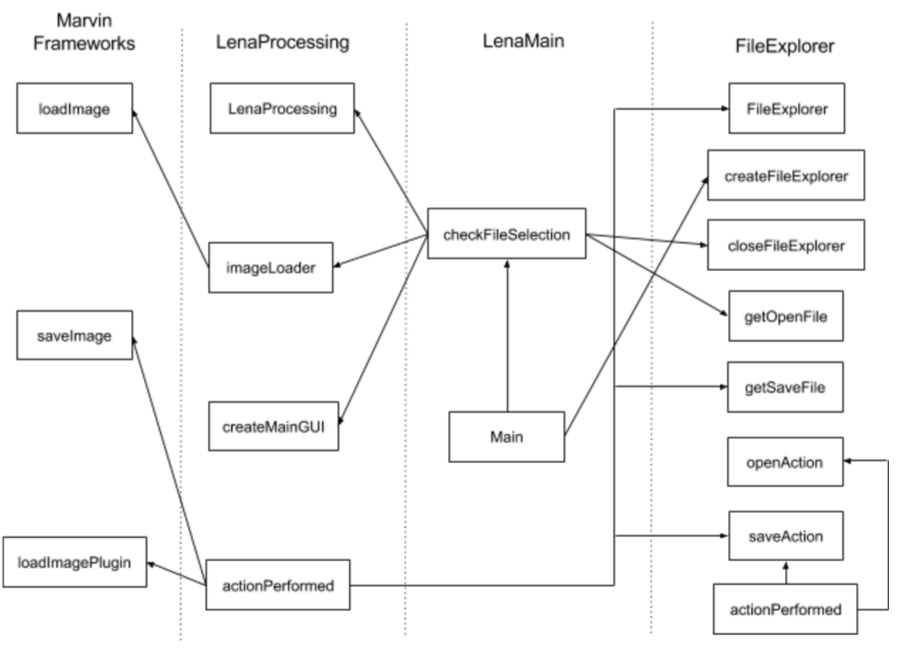
\includegraphics[width=0.7\textwidth]{Uses.png}
\caption{Use hierarchy among modules}
\label{FigUH}
\end{figure}

%\section*{References}

\bibliographystyle {plainnat}
\bibliography {MG}

\end{document}